\documentclass{standalone}
\usepackage{tikz}
\usepackage{pgfplots}

\begin{document}
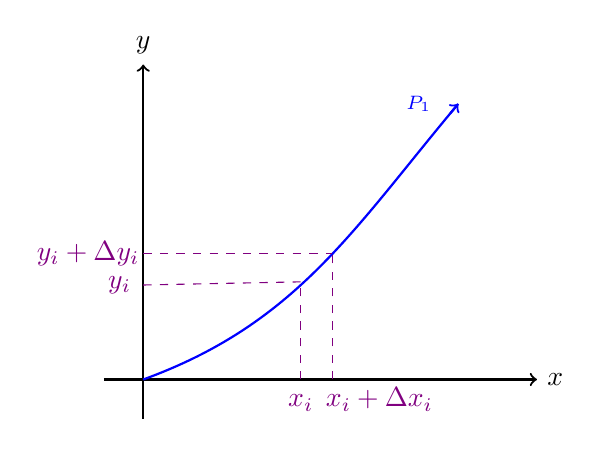
\begin{tikzpicture}[xshift=0cm, scale=1]

    % Axes with slightly extended lines to match the cross at origin in xbin
    \draw[thick,->] (-0.5,0) -- (5,0) node[right] {$x$}; % Extended x-axis left of origin
    \draw[thick,->] (0,-0.5) -- (0,4) node[above] {$y$}; % Aligned "y" label directly on top of the arrow
    
    % Inward concave curve (similar to red curve)
    \draw[thick,blue] (0,0) to [out=20,in=230] (4,3.5);
    
    % Arrow at the end of the curve
    \draw[thick,->,blue] (3.9,3.38) -- (4,3.5);
    
    % New dashed lines at x_i and x_i + Δx_i
    \draw[dashed, violet] (2,0) -- (2,1.2); % Dashed line at x_i
    \draw[dashed, violet] (2.4,0) -- (2.4,1.6); % Dashed line at x_i + Δx_i
    
    % New dashed lines for y_i and y_i + Δy_i
    \draw[dashed, violet] (0,1.2) -- (2,1.24); % Dashed line for y_i
    \draw[dashed, violet] (0,1.6) -- (2.4,1.6); % Dashed line for y_i + Δy_i
    
    % Labels
    \node[font=\scriptsize, color=blue] at (3.5, 3.5) {$P_1$};
    \node[color=violet] at (2, -0.3) {$x_i$};
    \node[color=violet] at (3, -0.2555) {$x_i + \Delta x_i$};
    \node[color=violet] at (-0.3, 1.2) {$y_i$};
    \node[color=violet] at (-0.7, 1.6) {$y_i + \Delta y_i$};
\end{tikzpicture}
\end{document}
